%======================================================================
\chapter{Observations}
%======================================================================

This would be a good place for some figures and tables.

Some notes on figures and photographs\ldots

\begin{itemize}
\item A well-prepared PDF should be 
  \begin{enumerate}
    \item Of reasonable size, {\it i.e.} photos cropped and compressed.
    \item Scalable, to allow enlargment of text and drawings. 
  \end{enumerate} 
\item Photos must be bit maps, and so are not scaleable by definition. TIFF and
BMP are uncompressed formats, while JPEG is compressed. Most photos can be
compressed without losing their illustrative value.
\item Drawings that you make should be scalable vector graphics, \emph{not} 
bit maps. Some scalable vector file formats are: EPS, SVG, PNG, WMF. These can
all be converted into PNG or PDF, that pdflatex recognizes. Your drawing 
package probably can export to one of these formats directly. Otherwise, a 
common procedure is to print-to-file through a Postscript printer driver to 
create a PS file, then convert that to EPS (encapsulated PS, which has a 
bounding box to describe its exact size rather than a whole page). 
Programs such as GSView (a Ghostscript GUI) can create both EPS and PDF from PS files.
Appendix~\ref{AppendixA} shows how to generate properly sized Matlab plots and save them as PDF.
\item It's important to crop your photos and draw your figures to the size that
you want to appear in your thesis. Scaling photos with the 
includegraphics command will cause loss of resolution. And scaling down 
drawings may cause any text annotations to become too small.
\end{itemize}
 
For more information on \LaTeX\, see the uWaterloo Skills for the Academic Workplace  \href{https://uwaterloo.ca/information-systems-technology/services/electronic-thesis-preparation-and-submission-support/ethesis-guide/creating-pdf-version-your-thesis/creating-pdf-files-using-latex/latex-ethesis-and-large-documents}{course notes}. 
\footnote{
Note that while it is possible to include hyperlinks to external documents,
it is not wise to do so, since anything you can't control may change over time. 
It \emph{would} be appropriate and necessary to provide external links to 
additional resources for a multimedia ``enhanced'' thesis. 
But also note that if the \package{hyperref} package is not included, 
as for the print-optimized option in this thesis template, any \cmmd{href} 
commands in your logical document are no longer defined.
A work-around employed by this thesis template is to define a dummy \cmmd{href} 
command (which does nothing) in the preamble of the document, 
before the \package{hyperref} package is included. 
The dummy definition is then redifined by the
\package{hyperref} package when it is included.
}

The classic book by Leslie Lamport \cite{lamport.book}, author of \LaTeX , is worth a look too, and the many available add-on packages are described by 
Goossens \textit{et al} \cite{goossens.book}.




Here is an example of how to include figures in \LaTeX. 
\Cref{fig:beam} shows a cantilever beam of circular cross-section
subjected to a point load and a uniformly distributed load, both of
which are uncertain. Note that it is better not to include the
extension of the figure's source file.

\begin{figure}[hbt]
  \centering
  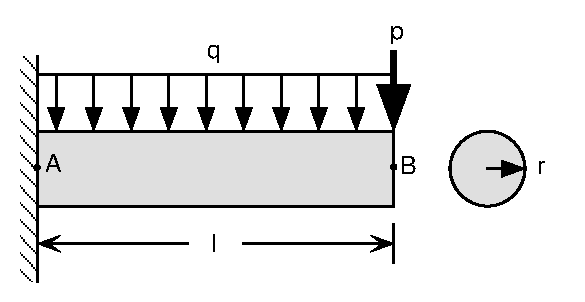
\includegraphics[clip=true]{figures/Inkscape/beam}
  \caption{Cantilever beam}
\label{fig:beam}
\end{figure}


\Cref{tab:prices,tab:team-sheet} show examples of how to add tables in \LaTeX.

\begin{table}[hbt]
  \centering
  \caption{Live stock prices}
  \label{tab:prices}
  \begin{tabular}{llr}  
    \toprule
    \multicolumn{2}{c}{Item} \\
    \cmidrule(r){1-2}
    Animal    & Description & Price (\$) \\
    \midrule
    Gnat      & per gram    & 13.65      \\
              &    each     & 0.01       \\
    Gnu       & stuffed     & 92.50      \\
    Emu       & stuffed     & 33.33      \\
    Armadillo & frozen      & 8.99       \\
    \bottomrule
  \end{tabular}
\end{table}


\begin{table}[hbt]
  \centering
  \caption{Team players}
  \label{tab:team-sheet}
  \begin{tabular}{ll}
    \toprule
    \multicolumn{2}{c}{Team sheet} \\
    \midrule
    GK & Paul Robinson \\
    LB & Lucas Radebe \\
    DC & Michael Duberry \\
    DC & Dominic Matteo \\
    RB & Dider Domi \\
    MC & David Batty \\
    MC & Eirik Bakke \\
    MC & Jody Morris \\
    FW & Jamie McMaster \\
    ST & Alan Smith \\
    ST & Mark Viduka \\
    \bottomrule
  \end{tabular}
\end{table}




Some examples of theorem-like environments. \Cref{def:prime} defines prime numbers. \Cref{cor:vertical-angles} is a consequence of \Cref{thm:one-side-line}.
%
\begin{definition}[Prime numbers]\label{def:prime}
  A prime number is a natural number that is only divisible by itself and 1.
\end{definition}
%
\begin{theorem}[Angles on one side of a line]\label{thm:one-side-line}
  Angles on one side of a straight line always add to \ang{180}.
\end{theorem}
%
\begin{corollary}[Vertical angles]\label{cor:vertical-angles}
  A corollary is a consequence of a theorem. 
  Following on from \Cref{thm:one-side-line} we find that where two lines intersect, opposite angles (also called Vertical Angles) are always equal.
\end{corollary}




